\documentclass{article}
\usepackage[utf8]{inputenc}
\usepackage{tikz, pgfplots, amsmath}
\usetikzlibrary{positioning,calc,arrows.meta}
\pgfplotsset{compat=1.18} 

\begin{document}
Hello

\vspace{1in}


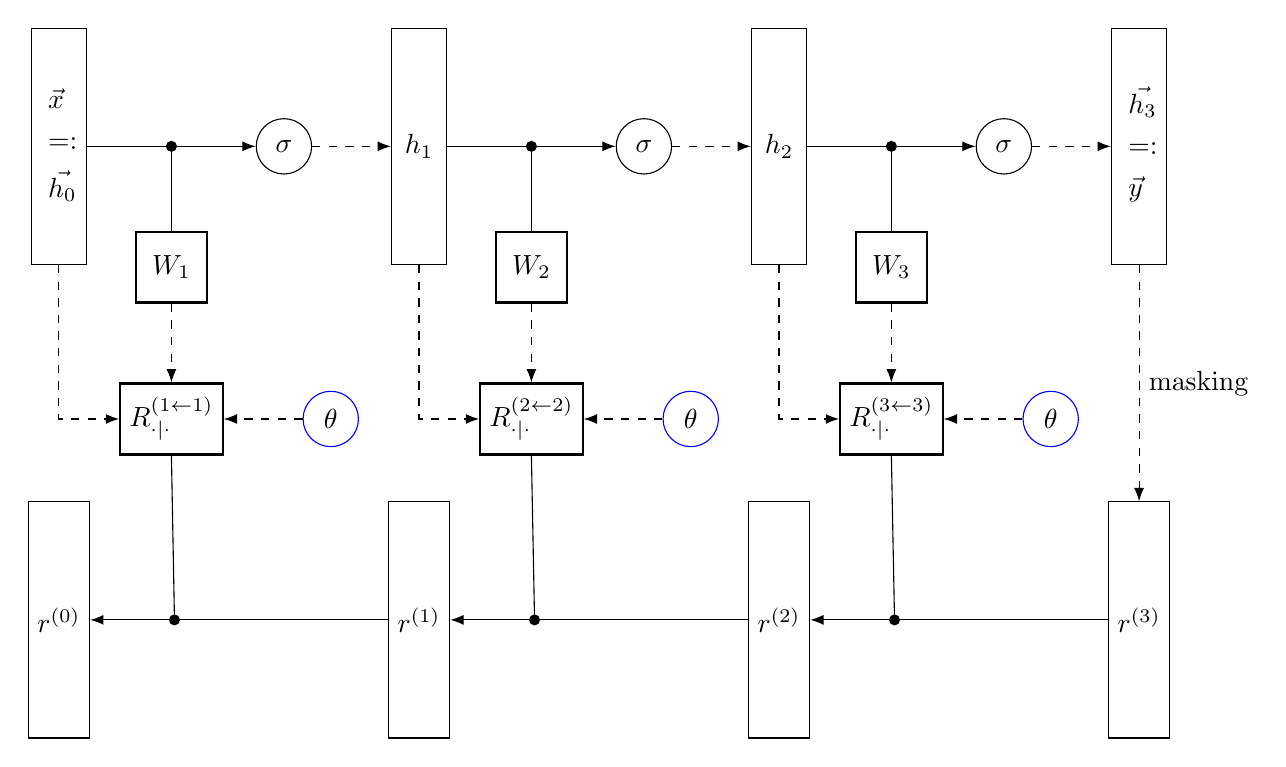
\begin{tikzpicture}[
    vec/.style={rectangle, draw=black, minimum size=7mm, minimum height=3cm},
    mat/.style={rectangle, thick, draw=black, minimum size=9mm, minimum height=9mm},
    meet/.style={circle, fill, minimum size=4pt, inner sep=0pt, outer sep=0pt},
    nonl/.style={circle, minimum size=20pt, draw=black},
    param/.style={circle, minimum size=20pt, draw=blue},
    ]
    \node[vec] (h_0) {
        $\begin{aligned}
            &\;\vec{x} \\ &=: \\ &\;\vec{h_0}
        \end{aligned}$
    };
    \node[meet, right=1cm of h_0] (m11) {};
    \node[nonl, right=1cm of m11] (nl1) {$\sigma$};
    \node[vec,  right=1cm of nl1] (h_1) {$h_1$};
    \node[meet, right=1cm of h_1] (m12) {};
    \node[nonl, right=1cm of m12] (nl2) {$\sigma$};
    \node[vec,  right=1cm of nl2] (h_2) {$h_2$};
    \node[meet, right=1cm of h_2] (m13) {};
    \node[nonl, right=1cm of m13] (nl3) {$\sigma$};
    \node[vec,  right=1cm of nl3] (h_3) {
        $\begin{aligned}
            &\;\vec{h_3} \\ &=: \\ &\;\vec{y}
        \end{aligned}$
    };

    \node[mat, below=1cm of m11] (W1) {$W_1$};
    \node[mat, below=1cm of m12] (W2) {$W_2$};
    \node[mat, below=1cm of m13] (W3) {$W_3$};

    % layer 1 arrows
    \draw[-]                    (h_0.east) to (m11);
    \draw[-]                    (W1.north) to (m11);
    \draw[-{LaTeX[]}]           (m11) to (nl1.west);
    \draw[-{LaTeX[]}, dashed]   (nl1.east) to (h_1.west);
    % layer 2 arrows
    \draw[-]                    (h_1.east) to (m12);
    \draw[-]                    (W2.north) to (m12);
    \draw[-{LaTeX[]}]           (m12) to (nl2.west);
    \draw[-{LaTeX[]}, dashed]   (nl2.east) to (h_2.west);
    % layer 3 arrows
    \draw[-]                    (h_2.east) to (m13);
    \draw[-]                    (W3.north) to (m13);
    \draw[-{LaTeX[]}]           (m13) to (nl3.west);
    \draw[-{LaTeX[]}, dashed]   (nl3.east) to (h_3.west);
    

    %%% LRP backwards matrix construction %%%
    % meeting points in second row
    % \node[meet, below=1cm of W1] (m21) {};
    % \node[meet, below=1cm of W2] (m22) {};
    % \node[meet, below=1cm of W3] (m23) {};

    % conditional relevancy matrices
    \node[mat, below=1cm of W1] (R1) {$R^{(1 \leftarrow 1)}_{\cdot | \cdot}$};
    \node[mat, below=1cm of W2] (R2) {$R^{(2 \leftarrow 2)}_{\cdot | \cdot}$};
    \node[mat, below=1cm of W3] (R3) {$R^{(3 \leftarrow 3)}_{\cdot | \cdot}$};

    % params
    \node[param, right=1cm of R1] (param1) {$\theta$};
    \node[param, right=1cm of R2] (param2) {$\theta$};
    \node[param, right=1cm of R3] (param3) {$\theta$};

    
    % layer 1 arrows
    \draw[-{LaTeX[]}, dashed]   (h_0.south) |- (R1.west);
    \draw[-{LaTeX[]}, dashed]   (W1.south)  to (R1.north);
    \draw[-{LaTeX[]}, dashed]   (param1.west) to (R1.east);
    % layer 2 arrows
    \draw[-{LaTeX[]}, dashed]   (h_1.south) |- (R2.west);
    \draw[-{LaTeX[]}, dashed]   (W2.south)  to (R2.north);
    \draw[-{LaTeX[]}, dashed]   (param2.west) to (R2.east);
    % layer 3 arrows
    \draw[-{LaTeX[]}, dashed]   (h_2.south) |- (R3.west);
    \draw[-{LaTeX[]}, dashed]   (W3.south)  to (R3.north);
    \draw[-{LaTeX[]}, dashed]   (param3.west) to (R3.east);


    %%% LRP backwards pass %%% 
    % relevancy vectors
    \node[vec,  below=3cm of h_0] (r_0) {$r^{(0)}$};
    \node[vec,  below=3cm of h_1] (r_1) {$r^{(1)}$};
    \node[vec,  below=3cm of h_2] (r_2) {$r^{(2)}$};
    \node[vec,  below=3cm of h_3] (r_3) {$r^{(3)}$};

    % meeting points in third row
    \node[meet, below=of R1, right=of r_0] (m31) {};
    \node[meet, below=of R2, right=of r_1] (m32) {};
    \node[meet, below=of R3, right=of r_2] (m33) {};

    % layer 1 arrows
    \draw[-]                    (r_1.west) to (m31);
    \draw[-]                    (R1.south) to (m31);
    \draw[-{LaTeX[]}]           (m31) to (r_0.east);
    % layer 2 arrows
    \draw[-]                    (r_2.west) to (m32);
    \draw[-]                    (R2.south) to (m32);
    \draw[-{LaTeX[]}]           (m32) to (r_1.east);
    % layer 3 arrows
    \draw[-]                    (r_3.west) to (m33);
    \draw[-]                    (R3.south) to (m33);
    \draw[-{LaTeX[]}]           (m33) to (r_2.east);

    % arrow to output layer relevancies
    \draw[-{LaTeX[]}, dashed]   (h_3.south) to node[right] {masking} (r_3.north);

    
\end{tikzpicture}

\vspace{1in}

% \begin{tikzpicture}
%     \node[draw] (a) {A};
%     \node[draw,right=of a] (b) {B};
%     \node[draw,below=5mm of b] (c) {C};

%     \path[-{LaTeX[]}] (b) edge (c);
%     \draw (a) |- ($(b)!0.42!(c)$);
% \end{tikzpicture}


\end{document}
